\documentclass[a4paper, twoside,openright]{article}
\usepackage[T1]{fontenc} % Font encoding, T1 = it
\usepackage[utf8]{inputenc} % Input encoding - per caratteri particolari
\usepackage[english,italian]{babel} % Lingua principale italiano, con parti in inglese
\usepackage{graphicx} % Per includere immagini esterne
\usepackage[a4paper,top=3cm,bottom=3cm,left=3cm,right=3cm]{geometry} %impaginazione e margini documento
\usepackage[fontsize=13pt]{scrextend} %dimensione font
\raggedbottom % Se la pagina non è completa, lascia lo spazio alla fine
\pagestyle{headings}
\usepackage{amsmath,amsthm,amssymb,mathtools,amsfonts}
\usepackage{enumitem} 
\usepackage{filecontents}
\usepackage{chngcntr}
\usepackage{ mathrsfs }
\usepackage{xcolor}
\usepackage{caption}
\captionsetup[figure]{labelformat=empty}
\usepackage[backend=bibtex]{biblatex}

\addbibresource{sample.bib}



\setlength{\parindent}{0pt}
\pagenumbering{arabic}

\newcommand{\ra}{\rightarrow}
\newcommand{\Ra}{\Rightarrow}
\newcommand{\LRa}{\Leftrightarrow}
\newcommand{\R}{\mathbb{R}}
\newcommand{\N}{\mathbb{N}}
\newcommand{\Q}{\mathbb{Q}}
\newcommand{\Z}{\mathbb{Z}}
\renewcommand{\P}{\mathbb{P}}
\renewcommand{\S}{\mathbb{S}}
\newcommand{\parti}{\mathcal{P}}
\newcommand{\fa}{\forall}
\newcommand{\fo}{\forall}
\newcommand{\e}{\varepsilon}
\newcommand{\<}{\langle}
\renewcommand{\>}{\rangle}

\DeclarePairedDelimiter{\abs}{\lvert}{\rvert}
\DeclarePairedDelimiter{\norm}{\lVert}{\rVert}

\newtheorem{teo}{Teorema}[]
\newtheorem{lemma}[teo]{Lemma}
\newtheorem{defin}[teo]{Definizione}
\newtheorem{cor}[teo]{Corollario}
\newtheorem{oss}[teo]{Osservazione}
\newtheorem{es}[teo]{Esempio}
\newtheorem{prop}[teo]{Proposizione}

% Bold math in titles
\makeatletter%
\DeclareRobustCommand*{\bfseries}{%
	\not@math@alphabet\bfseries\mathbf
	\fontseries\bfdefault\selectfont
	\boldmath
}
\makeatother

\counterwithin{teo}{section}

\begin{document}


% input file frontespizio.tex
\input{frontespizio}

\tableofcontents
\clearpage

\section{Introduzione}
	
	Nell’ambito della teoria della misura in $\R^n$, sono noti alcuni paradossi che mostrano come talvolta il comportamento della misura di Lebesgue possa essere controintuitivo.\\
	Un esempio famoso è il paradosso di Banach-Tarski, che utilizzando l’assioma della scelta per costruire insiemi non misurabili secondo Lebesgue, consente di decomporre la palla unitaria tridimensionale in finite parti, muoverle con movimenti rigidi e ricomporle, ottenendo due copie della palla iniziale.\\
	Tuttavia si possono ottenere risultati apparentemente paradossali anche restringendosi a considerare insiemi misurabili, ottenuti con metodi costruttivi che non richiedono l’uso dell’assioma della scelta.\\
	Un esempio è il seguente teorema, dimostrato da Davies nel 1952. \\
	Dato un insieme misurabile $A \subseteq \mathbb{R}^{2}$, esiste un insieme di rette $L$ tale che:\\
	- per ogni punto di $A$ passa una retta di $L$ (diremo che $L$ copre $A$);\\
	- l'insieme di punti coperto dalle rette di $L$ ha la stessa misura di Lebesgue di $A$.\\
	
	Se l’insieme $A$ è molto semplice, l’enunciato è intutivamente ovvio. Ad esempio se $A$ contiene un solo punto, basta prendere $L$ che contiene una sola retta, passante per quel punto. Diversamente, anche solo considerando $A$ uguale alla palla unitaria, l’enunciato di Davies non è più ovvio ma risulta paradossale. \\
	L’idea originale utilizzata da Davies per dimostrare il teorema era data dal seguente lemma, anch’esso difficilmente intuibile.\\
	Dato $\e >0$ e un compatto $K$ nel piano, esistono finiti parallelogrammi $P_1, P_2, …,P_n$ che coprono $K$ (cioè tali che $K \subseteq \bigcup_{i=1}^nP_i$) e per cui la misura di Lebesgue di $\bigcup_{i=1}^n P_i \setminus K$ è minore di $\e$. \\
	
	Costruzioni simili a quelle del teorema di Davies ammettono generalizzazioni in dimensione più alta e sono interessanti nell’analisi anche per la costruzione di controesempi.\\
	L’obiettivo di questa tesi è dare una dimostrazione del teorema di Davies, in una forma più generale. Tale dimostrazione, che non utilizza il precedente lemma, ripercorre e approfondisce invece il procedimento seguito da M. Cs\"{o}rnyei nei suoi articoli \Cite{1}, \cite{2}.\\
	
	Ricordiamo le seguenti definizioni.
	\begin{defin}
	Dato uno spazio di misura $(X, \mathcal{A})$, una misura $\mu$ si dice $\sigma$-finita se esistono degli insiemi $A_{1},A_{2},\ldots \in {\mathcal {A}}$ con $\mu \left(A_{n}\right)<\infty $ per ogni $n \in \N$, tali che $\bigcup _{n\in \mathbb {N} }A_{n}=X$.\\
	Se $X$ spazio topologico, una misura $\mu$ su $X$ si dice boreliana se ogni boreliano è $\mu$-misurabile. \\
	\end{defin}
	La generalizzazione cercata afferma che il teorema di Davies è valido per una generica misura boreliana $\sigma$-finita, in particolare quindi vale per la misura di Lebesgue.\\
	
	Il primo passo è mostrare un rafforzamento del teorema (nel caso della misura di Lebesgue e $A$ aperto). Per fare questo, si introduce una nozione di dualità che fa corrispondere a ogni retta un punto e viceversa. Questo consente di formulare il problema in forma duale, equivalente a quella iniziale, di più facile dimostrabilità.\\
	Per quest’ultima dimostrazione, saranno ampiamente utilizzate delle costruzioni puramente geometriche nel piano, che consentono di ottenere collezioni di parallelogrammi con caratteristiche utili ai fini della dimostrazione.\\
	Infine, la generalizzazione del teorema richiederà lo sviluppo di teoria più generale nell’ambito della teoria della misura, riguardante gli insiemi analitici o di Suslin.

	\newpage


\section{Misure su insiemi di rette}
Consideriamo l'insieme delle rette in $\P^2 \R$, dove ogni retta è descritta dall'equazione omogenea $ax_0+bx_1+cx_2=0$, per opportuni coefficienti $a,b,c$.\\
Possiamo identificare ogni retta con un punto di $\P^2 \R$, attraverso la bigezione $ax_0+bx_1+cx_2=0 \mapsto [a,b,c]$, che chiameremo corrispondenza duale.\\
Dato un insieme di rette proiettive, diciamo che questo è aperto, compatto, boreliano se il sottoinsieme di $\P^2 \R$ corrispondente nel duale lo è.\\

Si consideri il piano proiettivo reale $\P^2 \R$, realizzato come quoziente di $\S^2$ rispetto alla mappa $\pi$ che identifica i punti antipodali. Ogni misura su $\S^2$ induce tramite $\pi$ una misura su $\P^2\R$. Nel caso la misura su $\S^2$ sia misura usuale di area, chiameremo la misura immagine $\theta$.\\
Così, data una misura $\mu$ in $\P^2 \R$, si ha in modo naturale una misura $\tilde \mu$ sulle rette proiettive. In particolare, diciamo che un insieme di rette è misurabile rispetto a $\tilde \mu$ se l'insieme di punti duale lo è rispetto a $\mu$.\\

Data una retta affine in $\R^2$, si può omogeneizzare l'equazione che la descrive, associando a $a+bx+cy=0$ l'equazione omogenea $ax_0+bx_1+cx_2=0$, e assumere che questa retta sia in $\P^2 \R$. Si definisce così una misura anche sulle rette affini.\\
Come prima si può parlare di insiemi di rette affini aperti, compatti, boreliani, misurabili.

\begin{oss}
	\label{osservazione}
	Un insieme di rette passanti per un punto $P \in \P^2 \R$, è rappresentato nel duale da punti appartenenti a una retta $\ell_P$.\\
	Infatti, se $P=[a,b,c]$, una retta passante per $P$ soddisfa $ax_0+bx_1+cx_2=0$. Tale retta è rappresentata da $[x_0,x_1,x_2]$, che quindi appartiene alla retta $az_0+bz_1+cz_2=0$.\\
	In particolare, $\ell_P$ è rappresentata nel duale dal punto $P$.
\end{oss}

Fissato un punto $P$ nel piano proiettivo, la misura $\tilde \theta$ delle rette passanti per esso è sempre nulla, perché un'insieme lineare in $\P^2 \R$ ha area nulla.\\
Usando l'osservazione, si può comunque definire una misura sulle rette passanti per $P$: è quella indotta dalla naturale misura di lunghezza sulla retta proiettiva $\ell_P$ (omeomorfa a $\S^1$ quozientato).

\begin{defin}
Una direzione è un punto all'infinito della chiusura proiettiva di $\R^2$. La misura sulle direzioni è data dalla misura di lunghezza sulla retta all'infinito.\\
Dato un insieme di rette $L$ in $\R^2$ e una direzione $d$, sia $L_{d}$ l'insieme delle rette di $L$ in direzione $d$.
\end{defin}

A meno passare alle chiusura proiettiva, $L_{d}$ è un sottoinsieme di rette passanti per un fissato punto all'infinito $Q$.\\
Come prima, la misura $\tilde \theta$ di $L_d$ è nulla, ma esiste una misura su tale insieme, indotta dalla misura lineare su $\ell_Q$.\\
Si osserva che $L_d$ è trascurabile rispetto a questa misura se e solo se per ogni $t_d$ retta ortogonale alla direzione $d$, $ (\bigcup L_d) \cap t_d$ ha misura lineare nulla.\\
Inoltre vale il seguente lemma.

\begin{lemma}
	Un insieme misurabile di rette $L$ nel piano ha misura $\tilde \theta$ nulla se e solo se contiene trascurabili rette in quasi ogni direzione. 
\end{lemma}

\begin{proof}
	Ogni insieme misurabile $A \subseteq \R^2$ ha misura nulla se e solo se esiste $x \in \R^2$ (equivalentemente, per ogni $x$), quasi ogni retta per $x$ interseca $A$ in insieme di misura lineare nulla. Infatti segue subito applicando il teorema di Fubini e un cambio di variabili in coordinate polari nel piano.\\
	Posso supporre che $L$ sia un insieme di rette proiettive, rappresentato nel duale dai punti $A$.\\
	Fissiamo $x$ punto nel duale, che corrisponde alla retta all'infinito.\\
	Passando in carte, posso supporre che $x \in \R^2$ e $A\subseteq \R^2$, a meno di un insieme di misura nulla.\\
	$\tilde \theta (L)=0 \LRa \theta(A)=0 \LRa$ per quasi ogni retta $\ell$ per $x$, $\theta(\ell \cap A)=0$.\\
	Passando al duale, questo avviene se e solo se per quasi ogni punto all'infinito (direzione), la misura delle rette di $L$ passanti per quel punto (in quella direzione) è nulla.
\end{proof}	



	
\newpage

\section{Il Teorema di Davies per la misura di Lebesgue}

Procediamo con la dimostrazione di lemma che implica il teorema di Davies nel caso della misura di Lebesgue e $A$ aperto.\\
Premettiamo alcune definizioni e proprietà.

\begin{defin}
Per un insieme di rette $L$ nel piano $\R^2$, sia $L^{*}= \{\bigcup \ell | \ell \in L\}$, cioè i punti di $\R^2$ coperti da rette di $L$; per un insieme di punti $A \subseteq \R^2$, sia $A^{*}$ l'insieme delle rette per i punti di $A$.
\end{defin}

\begin{defin}
	Un insieme è residuale se il suo complementare è di prima categoria. Un insieme è di prima categoria se unione numerabile di insiemi mai densi (cioè con chiusura a parte interna vuota).
\end{defin}

\begin{prop} \label{prop}
	Sono vere le seguenti proprietà:
	\begin{itemize}
		\item ogni soprainsieme di un insieme residuale è residuale. In particolare, l'unione arbitraria di insiemi residuali è residuale.
		\item l'intersezione numerabile di insiemi residuali, è residuale. Inoltre l'intersezione numerabile di aperti densi è un insieme residuale.
	\end{itemize}
\end{prop}
\begin{proof}
	Passando al complementare, sia $A$ di prima categoria e $B \subseteq A$. Vale $A= \bigcup_n U_n$, con gli $U_n$ mai densi.\\
	Allora $B= \bigcup_n(B \cap U_n)$, cioè è unione numerabile di insiemi mai densi.\\
	Sia ora $A=\bigcup_nA_n$, con $A_n$ di prima categoria per ogni $n$, cioè $A_n$ è unione numerabile di insiemi mai densi. Allora anche $A$ è unione numerabile di insiemi mai densi.\\
	Mostriamo infine che un aperto denso è residuale. Infatti il suo complementare è un chiuso a parte interna vuota.	
\end{proof}

\begin{lemma} \label{lemma1}
Sia $A$ aperto del piano e sia $x$ un punto che non appartiene ad $A$. Allora esiste un insieme boreliano di rette $L$ tale che:
\begin{itemize}
	\item per ogni punto $p \in A$, l'insieme delle rette di $L$ passanti per $p$ è residuale nell'insieme delle rette per $p$;
	\item $L^{*} \backslash A$ interseca ogni retta per $x$ in un insieme di misura di Lebesgue nulla.
\end{itemize}
\end{lemma}

Ricordiamo che, per Fubini, il sottoinsieme del piano $L^* \setminus A$ ha misura di Lebesgue nulla se e solo se, dato un punto $x$, \emph{quasi} ogni retta per $x$ interseca $L^* \setminus A$ in un insieme di misura lineare nulla.\\
Il lemma richiede non solo che $L^* \setminus A$ abbia misura nulla, ma anche che intersechi ogni retta per un dato punto in un insieme di misura lineare nulla. \\
Inoltre è la condizione di residualità implica che $L$ copre $A$. Infatti preso un punto di $A$, per il teorema di Baire, se l'insieme di rette di $L$ passanti per esso è residuale, allora è non vuoto.\\

In questo lemma, i punti e le rette in questione sono affini. Quindi per definire la versione duale del lemma, bisogna dare una formulazione "proiettiva" equivalente, immergendo $\R^2$ in $\P^2\R$. Si ammette che $A$ possa avere punti all'infinito e che $L$ possa contenere la retta all'infinito. Si richiede che $x$ non sia all'infinito. Inoltre, la misura di Lebesgue sulla retta è sostituta dalla misura di lunghezza su una retta proiettiva.\\
Questa operazione è possibile perché:
\begin{itemize}
	\item la nozione di misura nulla su una retta è ben definita: con le definizioni date, un sottoinsieme di una retta proiettiva ha misura nulla se e solo se la sua parte affine ha misura di Lebesgue nulla. 
	\item si aggiunge a $L$ al più una retta, quindi la condizione di residualità è invariata.
	\item si aggiungono a $L^* \setminus A$ al più i punti della retta all'infinito. Quindi, data una retta proiettiva passante per $x$, la nozione di trascurabilità della sua intersezione con $L^* \setminus A$ rimane invariata.
\end{itemize}
Dopo queste osservazioni, ha senso la formulazione duale del lemma, come segue 

\begin{lemma} \label{lemma2}
Sia $L$ un insieme aperto di rette e sia $X$ un retta non appartenente a $L$. Allora esiste un insieme boreliano di punti $A$ per cui:

\begin{itemize}
	\item ogni retta $\ell \in L$ interseca $A$ in un insieme residuale, cioè $\ell \cap A$ residuale in $\ell$;
	\item per ogni punto di $X$ passano trascurabili rette di $A^{*} \backslash L$.
\end{itemize}
\end{lemma}

	Si mostra facilmente che la formulazione duale è equivalente a quella data inizialmente. Mostriamo l'implicazione utile a noi, introducendo prima la seguente notazione.\\
	Dato un punto $p$, sia $p^*$ l'insieme delle rette passanti per $p$. Data una retta $\ell$, sia $\ell^*$ l'insieme dei punti passanti per $\ell$.\\
	Indichiamo con $\lambda$ la misura lineare su una retta proiettiva.
	
\begin{proof} [Dimostrazione del lemma \ref{lemma1}]
	Sia $M$ l'aperto di rette corrispondente nel duale ad $A$ e $X$ la retta proiettiva corrispondente a $x$. Applicando il lemma \ref{lemma2} a questi, esiste un insieme boreliano di punti $B$ per cui:
	\begin{itemize}
		\item $\fa \ell \in M, \ell^* \cap B$ è residuale;
		\item $\fa p \in X, \lambda((B^* \setminus M) \cap p^*)=0$
	\end{itemize}
	Chiamando $L$ l'insieme di rette che rappresenta nel duale $B$, valgono le seguenti:
	\begin{itemize}
		\item 	$\fa p \in A, p^* \cap L$ è residuale;
		\item 	$\fa \ell \ni x, \lambda((L^* \setminus A) \cap \ell^*)=0$
	\end{itemize}
\end{proof}

Possiamo assumere che $X$ sia la retta all'infinito. Allora i punti di $X$ sono direzioni di rette nel piano e le rette di $L$ sono tutte affini. Possiamo formulare il lemma \ref{lemma2} in una versione equivalente.

\begin{lemma} \label{lemma2bello}
Sia $L$ un insieme aperto di rette, allora esiste un insieme di punti $A$ tale che:
\begin{itemize}
	\item ogni retta di $L$ interseca $A$ in un insieme residuale;
	\item in ogni direzione ci sono trascurabili rette di  $A^{*} \backslash L$.
\end{itemize}
\end{lemma}

Per dimostrarlo, usiamo il seguente lemma, la cui dimostrazione è riportata nell'ultima sezione.\\
Introduciamo anche la seguente notazione. Per un dato parallelogramma $P$, aperto e non degenere, e un intervallo di direzioni $I$, sia $A_{P, I}$ l'insieme di rette per i punti di $P$ in direzioni appartenenti a $I$.\\
Inoltre, d'ora in poi, ogni parallelogramma nel piano si intende aperto, come anche ogni intervallo di direzioni di rette nel piano.

\begin{lemma} \label{lemmabrutto}
Per ogni parallelogramma $P$, numero positivo $\varepsilon$ e intervalli di direzioni $I, J$ tale che $\operatorname{cl}(I) \subseteq J$, esistono dei sotto parallelogrammi $P_{1}, P_{2}, \ldots$ tali che:
\begin{itemize}
	\item ogni retta che interseca $P$ e la cui direzione appartiene a $I$ interseca anche uno dei parallelogrammi, cioè $\bigcup_{n} A_{P_{n}, I}=A_{P, I}$;
	\item la proiezione di $\bigcup_{n} P_{n}$ ha misura di Lebesgue minore di $\varepsilon$ in ogni direzione non appartenente a $J$.
\end{itemize}
\end{lemma}

\begin{proof}[Dimostrazione del lemma \ref{lemma2bello}]
Per ogni successione finita di naturali $\mathbf{n}$, scegliamo $\varepsilon_{\mathbf{n}}$ positivo tale che, per ogni $k$ naturale positivo, $\sum_{\mathbf{n}=n_{1} n_{2} \cdots n_{k}} \varepsilon_{\mathbf{n}}<1 / 2^{k}$.\\
Siano $P_{1}, P_{2}, \ldots$ parallelogrammi e siano $I_{1}, I_{2}, \ldots$ intervalli di direzioni, tali che $A_{P_{j}, I_{j}} \subseteq L$ per ogni $j$ e, per ogni retta $\ell \in L$, l'insieme $\left\{P_{j}: \ell \in A_{P_{j}, I_{j}}\right\}$ sia un ricoprimento di Vitali di $\ell$, cioè ogni punto di $\ell$ sia coperto da un parallelogramma di diametro arbitrariamente piccolo. In particolare data $\ell \in L$, $ \bigcup_j P_j \cap \ell = \ell $.\\
L'esistenza di una configurazione di questo tipo è garantita perché $L$ è aperto. Infatti, supponiamo $\ell$ non verticale e sia $x_{\ell}$ il punto che rappresenta $\ell$ nel duale. Allora esiste un intorno di $x_{\ell}$ contenuto in $L$, i cui punti corrispondono a rette in un certo intervallo di direzioni e passanti per un fissato segmento verticale. Questo consente di scegliere opportunamente i $P_i$ per ricoprire ogni retta $\ell \in L$. La richiesta che il ricoprimento sia di Vitali è facilmente realizzabile.\\

Vogliamo costruire induttivamente una collezione numerabile di parallelogrammi indicizzata dalle sequenze finite di naturali. Sempre induttivamente, a ogni parallelogramma $P_{\mathbf{n}}$ associo degli intervalli di direzioni $I_{\mathbf{n}}, J_{\mathbf{n}}$.\\
I parallelogrammi $P_1, P_2,...$, indicizzati da sequenze finite di lunghezza 1, sono il passo base dell'induzione, con intervalli $I_1, I_2,...$ e con $J_1=J_2=...$ che contengono tutte le direzioni.\\
Per il passo induttivo, sia $\mathbf{n}=n_{1} n_{2} \cdots n_{k}$ una sequenza finita di naturali di lugnhezza $k$. Supponiamo che siano già stati definiti $P=P_{\mathbf{n}}$, $I=I_{\mathbf{n}}$, $J=J_{\mathbf{n}}$, allora definiamo $P_{\mathbf{n} j}, I_{\mathbf{n} j}, J_{\mathbf{n} j}$ per ogni $j \in \mathbb{N}$ positivo come segue.\\

Scegliamo dei sotto-parallelogrammi $P^{1}, P^{2}, \ldots$ di $P=P_{\mathbf{n}}$ e dei sotto-intervalli $I^{1}, I^{2}, \ldots$ di $I=I_{\mathbf{n}}$ con $\operatorname{cl}(I^j) \subseteq I$ tali che per ogni $\ell \in A_{P, I}$, l'insieme di sotto-parallelogrammi $\left\{P^{j}: \ell \in A_{P^{j}, I^{j}}\right\}$
sia un ricoprimento di Vitali del segmento $\ell \cap P$. \\
Per ogni $j$ naturale positivo, scegliamo  $\varepsilon^{j} >0$ in modo che $\sum_j \e^j < \e_{\mathbf{n}}$ e un intervallo di direzioni $J^{j} \subseteq I$ tale che $\operatorname{cl}\left(I^{j}\right) \subseteq J^{j}$ e $\left|J^{j} \backslash I^{j}\right|<\varepsilon_\mathbf{n}$, dove intendiamo l'usuale misura di lunghezza sull'insieme delle direzioni.\\ 
Applichiamo il lemma \ref{lemmabrutto} a tutti i parallelogrammi $P^{j}$, con intervalli $I^{j}, J^{j}$ e numeri $\varepsilon^{j}$. Otteniamo un insieme numerabile di sotto-parallelogrammi di $P$, che chiameremo $P_{\mathbf{n} 1}, P_{\mathbf{n} 2}, \ldots$. Se il parallelogramma $P_{\mathbf{n} m}$ è ottenuto applicando il lemma \ref{lemmabrutto} a $P^{j}, I^{j}, J^{j}, \varepsilon^{j}$, allora poniamo $I_{\mathbf{n} m}=I^{j}$ e $J_{\mathbf{n} m}=J^{j}$.\\

Sia $\ell \in L$ e $P=P_{\mathbf{n}}$, ricordiamo che l'insieme $\left\{P^{j}: \ell \in A_{P^{j}, I^{j}}\right\}$ è un ricoprimento di Vitali di $\ell \cap P$ per ogni $\ell \in A_{P^, I}$. In particolare, dato un punto $x \in \ell \cap P$, allora $x \in P^j$ per un certo $j$ e la direzione di $\ell$ appartiene a $I_j$.\\
Ma per il primo punto del lemma \ref{lemmabrutto}, se $\ell$ interseca $P^j$ e la sua direzione appartiene a $I_j$, allora interseca uno dei sotto-parallelogrammi ottenuti applicando il lemma a $P^{j}, I^{j}, J^{j}, \varepsilon^{j}$.\\
Ricordando che il ricoprimento è di Vitali, si può anche richiedere che $P^j$ come sopra abbia diametro piccolo a piacere.\\
Quindi esiste un parallelogramma $P_{\mathbf{n}m}$, ottenuto da $P^j$, arbitrariamente vicino a $x$ e che interseca $\ell$. Quindi l'insieme $\left\{P_{\mathrm{n} m}: \ell \in A_{P_{\mathrm{n}m}, I_{\mathrm{n} m}}\right\}$
copre un sottoinsieme aperto denso del segmento $\ell \cap P$. In particolare, $\bigcup_m P_{\mathbf{n}m} \cap \ell$ è denso in $P_\mathbf{n} \cap \ell$.\\
Ricordiamo che data $\ell \in L$ allora $ \bigcup_j P_j \cap \ell = \ell $, quindi $\bigcup_{\mathbf{n}=n_{1} n_{2} \cdots n_{k}} P_{\mathbf{n}}$ interseca ogni retta $\ell \in L$ in un insieme aperto denso.\\
Per il terzo punto della proposizione \ref{prop}, l'insieme 
$$
A:= \bigcap_{k} \bigcup_{\mathbf{n}} P_{\mathbf{n}=n_{1} n_{2} \cdots n_{k}}
$$
interseca ogni retta $\ell \in L$ in un insieme residuale, quindi soddisfa la prima condizione del lemma \ref{lemma2bello}.\\
Notiamo che $A$ è intersezione numerabile di aperti, quindi è boreliano.\\

Mostriamo che anche la seconda condizione è soddisfatta.\\
Se $\ell \notin L$, si hanno due possibilità: o $\ell$ non interseca $P_{\mathbf{n}}$ per ogni sequenza $\mathbf{n}$, oppure esiste $P_\mathbf{n}$ intersecato da $\ell$.\\
Nel primo caso, $\ell$ non interseca $A$.\\
Nel secondo caso, ricordiamo che $A_{P_\mathbf{n},I_\mathbf{n}} \subseteq L$, quindi la direzione $d$ di $\ell$ non appartiene a $I_{\mathbf{n}}$. Posso supporre che $d$ non appartenga neanche a $\operatorname{cl}(I_\mathbf{n})$: altrimenti basta prendere un parallelogramma $P_{\mathbf{n}m} \subseteq P_{\mathbf{n}}$ che interseca $\ell$ e, siccome $\operatorname{cl}(I_{\mathbf{n}m}) \subseteq I_{\mathbf{n}}$, $d \not \in \operatorname{cl}(I_{\mathbf{n}m})$.\\
Quindi la distanza della direzione $d$ da $\operatorname{cl}(I_\mathbf{n})$ è maggiore di $\delta$ per un certo $\delta >0$.\\
Ricordiamo che, $|J_{\mathbf{n}m} \setminus I_{\mathbf{n}m}| < \e_{\mathbf{n}}$ per ogni $m$ e che $\e_{\mathbf{n}} < 1/2^k$. Quindi, per $r$ abbastanza grande, $|J_{\mathbf{n} m_{1} \cdots m_{r}} \setminus I_{\mathbf{n} m_{1} \cdots m_{r}}| < \e_{\mathbf{n} m_{1} \cdots m_{r-1}} < 1/2^{k+r-1}<\delta$.\\
Se $d \not \in I_{\mathbf{n}} $, allora $d \not \in \bigcup_{m_{1} m_{2} \cdots m_{r}} I_{\mathbf{n} m_{1} \cdots m_{r}} \subseteq I_{\mathbf{n}}$, quindi esiste un intero positivo positivo $r_0$ per cui la direzione di $\ell$ non appartiene a $\bigcup_{m_{1} m_{2} \cdots m_{r}} J_{\mathbf{n} m_{1} \cdots m_{r}}$ per ogni $r \geq r_0$.\\
Per tali valori di $r$, ricordando il secondo punto del lemma \ref{lemmabrutto} e la sommabilità degli $\e^j$ come sopra, si ha che la proiezione ortogonale di $\bigcup_{m_{1} m_{2} \cdots m_{r}} P_{\mathbf{n} m_{1} \cdots m_{r}}$ nella direzione di $\ell$ ha misura minore o uguale a $\sum_{m_{1} m_{2} \cdots m_{r-1}} \varepsilon_{\mathbf{n} m_{1} \cdots m_{r-1}}$.\\
Tale somma per ipotesi è minore di $1/2^{k+r-1}$. Quindi la proiezione ortogonale di $\bigcap_{r} \bigcup_{m_{1} m_{2} \cdots m_{r}} P_{\mathbf{n} m_{1} \cdots m_{r}} $ lungo $\ell$ ha misura nulla.\\
Consideriamo ora tutte le rette non in $L$, in una direzione fissata $d$, che intersecano $A$. Siano $P_{\mathbf{n}_1}, P_{\mathbf{n}_2},...$ i parallelogrammi che queste intersecano.\\
Per mostrare che le rette non in $L$ in direzione $d$ che intersecano $A$ hanno misura nulla, è sufficiente mostrare che l'insieme $\bigcap_r \bigcup_i \bigcup_{m_1 ... m_r}  P_{\mathbf{n}_i m_{1} ...m_{r} } \subseteq A$ ha proiezione di misura nulla in direzione $d$. Ma tale insieme è uguale a $\bigcup_i \bigcap_r \bigcup_{m_1 ... m_r}  P_{\mathbf{n}_i m_{1} ...m_{r} }$ e verifica la richiesta per quanto precedentemente mostrato applicato a ogni $\mathbf{n}_i$.
\end{proof}

\newpage

\section{Problema della misurabilità di $L^*$ e teoria di Suslin}

Nel tentativo di generalizzare il teorema per una misura boreliana $\sigma$-finita $\mu$, si chiede che, dato un insieme di rette $L$ boreliano, l'insieme di punti $L^*$ coperto da tali rette sia misurabile rispetto a $\mu$.\\
La dimostrazione di questo fatto richiede l'introduzione di alcuni concetti più generali nell'ambito della teoria della misura.

\begin{defin}
	Sia $X$ un insieme non vuoto e sia $\mathcal{E}$ una collezione di suoi sottoinsiemi. Diciamo che $\left\{A_{n_{1}, \ldots, n_{k}}\right\}$ è uno schema di Suslin a valori in $\mathcal{E}$ se, per ogni sequenza finita di naturali $\left(n_{1}, \ldots, n_{k}\right)$, si ha $A_{n_{1}, \ldots, n_{k}} \in \mathcal{E}$.\\
	L'operazione di Suslin (o A-operazione) in $\mathcal{E}$ associa a ogni schema di Suslin $\left\{A_{n_{1}, \ldots, n_{k}}\right\}$ a valori in $\mathcal{E}$ l'insieme
	$$
	A=\bigcup_{\left(n_{i}\right) \in \mathbb{N}^{\infty}} \bigcap_{k=1}^{\infty} A_{n_{1}, \ldots, n_{k}} .
	$$
	Gli insiemi in questa forma sono detti di $\mathcal{E}$-Suslin o $\mathcal{E}$-analitici. \\
	La collezione degli insiemi di questo tipo e l'insieme vuoto è indicata con $S(\mathcal{E})$.
\end{defin}	

Diciamo che uno schema di Suslin è monotono (o regolare) se $A_{n_{1}, \ldots, n_{k}, n_{k+1}} \subseteq A_{n_{1}, \ldots, n_{k}}$ per ogni $k$ e per ogni successione $(n_i)$.\\
Se $\mathcal{E}$ è chiuso per intersezione finita, allora uno schema di Suslin $\left\{A_{n_{1}, \ldots, n_{k}}\right\}$ a valori in $\mathcal{E}$ può essere sostituito da uno schema monotono $\left\{A^*_{n_{1}, \ldots, n_{k}}\right\}$ che dà lo stesso risultato applicando l'operazione di Suslin. Infatti basta porre 
$$
A_{n_{1}, \ldots, n_{k}}^{*}:=A_{n_{1}} \cap A_{n_{1}, n_{2}} \cap \cdots \cap A_{n_{1}, \ldots, n_{k}} .
$$

Mostriamo ora il seguente lemma, dove con $\left(\mathbb{N}^{\infty}\right)^{\infty}$ indichiamo lo spazio delle successioni $\eta=\left(\eta^{1}, \eta^{2}, \ldots\right)$ con $\eta^{i} \in \mathbb{N}^{\infty}$.

\begin{lemma}
	Esistono delle bigezioni
	$$	\beta: \mathbb{N} \times \mathbb{N} \rightarrow \mathbb{N} \quad \text { and } \quad \Psi: \mathbb{N}^{\infty} \times\left(\mathbb{N}^{\infty}\right)^{\infty} \rightarrow \mathbb{N}^{\infty}
	$$
	tali che per ogni $m, n \in \mathbb{N}, \sigma=\left(\sigma_{i}\right) \in \mathbb{N}^{\infty}$ e $\left(\tau^{i}\right) \in\left(\mathbb{N}^{\infty}\right)^{\infty}$, dove $\tau^{i}=\left(\tau_{j}^{i}\right) \in \mathbb{N}^{\infty}$, le collezioni $\sigma_{1}, \ldots, \sigma_{m}$ e $\tau_{1}^{m}, \ldots, \tau_{n}^{m}$ sono univocamente determinate dalle prime $\beta(m, n)$ componenti di $\Psi\left(\sigma,\left(\tau^{i}\right)\right)$.
\end{lemma}	

\begin{proof}
	Sia $\beta(m, n)=2^{m-1}(2 n-1)$. Allora $\beta$ è una bigezione da $\mathbb{N} \times \mathbb{N}$ in $\mathbb{N}$ (per unicità della fattorizzazione dei naturali). Siano $\varphi(l):=m, \psi(l):=n$, dove $\beta(m, n)=l$. Siano $\sigma=\left(\sigma_{i}\right) \in \mathbb{N}^{\infty}$ e $\left(\tau^{i}\right) \in\left(\mathbb{N}^{\infty}\right)^{\infty}$, con $\tau^{i}=\left(\tau_{j}^{i}\right) \in \mathbb{N}^{\infty}$. Poniamo
	$$
	\Psi\left(\sigma,\left(\tau^{i}\right)\right)=\left(\beta\left(\sigma_{1}, \tau_{\psi(1)}^{\varphi(1)}\right), \ldots, \beta\left(\sigma_{l}, \tau_{\psi(l)}^{\varphi(l)}\right), \ldots\right) .
	$$
	Allora per ogni $\eta=\left(\eta_{i}\right) \in \mathbb{N}^{\infty}$, l'equazione $\Psi\left(\sigma,\left(\tau^{i}\right)\right)=\eta$ ha a soluzione unica $\sigma_{i}=\varphi\left(\eta_{i}\right),  \tau_{\psi(i)}^{\varphi(i)}=\psi(\eta_i)$ da cui $\tau_{j}^{i}=\psi\left(\eta_{\beta(i, j)}\right)$. Quindi $\Psi$ è bigettiva.\\
	Poiché $m \leq \beta(m, n)$ e $\beta(m, k) \leq \beta(m, n)$ per $k \leq n$, dalla scrittura esplicita delle soluzioni $\sigma, (\tau^i)$ segue che le prime $\beta(m, n)$ componenti di $\Psi\left(\sigma,\left(\tau^{i}\right)\right)$ determinano univocamente le prime $m$ componenti di $\sigma$ e le prime $n$ componenti di $\tau^{m}$.
	
\end{proof}

Ora usiamo il precedente lemma per mostrare una proprietà generale degli insiemi di Suslin.\\

\begin{teo} \label{SE}
	\hfill
	\begin{itemize}
		\item $S(S(\mathcal{E}))=S(\mathcal{E})$. In particolare, la classe $S(\mathcal{E})$ è chiusa per unioni e intersezioni numerabili.
		\item Se il complementare di ogni insieme in $\mathcal{E}$ appartiene a $S(\mathcal{E})$ (ad esempio se è unione numerabile di elementi di $\mathcal{E}$) e $\varnothing \in \mathcal{E}$, allora la $\sigma$-algebra $\sigma(\mathcal{E})$ generata da $\mathcal{E}$ è contenuta in $S(\mathcal{E}).$
	\end{itemize}
\end{teo}

\begin{proof}
	Ovviamente $S(\mathcal{E}) \subseteq S(S(\mathcal{E}))$. Per l'altra inclusione, siano $A_{n_{1}, \ldots, n_{k}}^{\nu_{1}, \ldots, \nu_{m}} \in \mathcal{E}$ e siano
	$$ A_{n_{1}, \ldots, n_{k}}=\bigcup_{(\nu_j) \in \mathbb{N}^{\infty}} \bigcap_{m=1}^{\infty} A_{n_{1}, \ldots, n_{k}}^{\nu_{1}, \ldots, \nu_{m}} \text {. }	$$
	$$	A=\bigcup_{\left(n_{i}\right) \in \mathbb{N}^{\infty}} \bigcap_{k=1}^{\infty} A_{n_{1}, \ldots, n_{k}} \in S(S(\mathcal{E}))$$
	
	Con la stessa notazione di cui sopra, siano $\eta_{1}, \ldots, \eta_{l}$ naturali fissati. Per suriettività di $\Psi$, esistono $\sigma \in \mathbb{N}^{\infty}$ e $\tau=\left(\tau^{m}\right) \in\left(\mathbb{N}^{\infty}\right)^{\infty}$ tali che $\eta_{1}=\Psi(\sigma, \tau)_{1}, \ldots, \eta_{l}=$ $\Psi(\sigma, \tau)_{l}$. Anche se $\sigma$ e $\tau$ non sono univocamente determinate, per il lemma precedente, le collezioni $\sigma_{1}, \ldots, \sigma_{\varphi(l)}$ e $\tau_{1}^{\varphi(l)}, \ldots, \tau_{\psi(l)}^{\varphi(l)}$ lo sono. Ha senso quindi porre
	$$
	B\left(\eta_{1}, \ldots, \eta_{l}\right)=A_{\sigma_{1}, \ldots, \sigma_{\varphi(l)}}^{\tau_{1}^{\varphi(l)}, \ldots, \tau_{\psi(l)}^{\varphi(l)}} \in \mathcal{E} .
	$$
	Sia $\eta=\left(\eta_{l}\right)\in \N^{\infty}$. Mostriamo che $A=\bigcup_{\eta} \bigcap_{l=1}^{\infty} B\left(\eta_{1}, \ldots, \eta_{l}\right) \in S(\mathcal{E})$, quindi che $S(S(\mathcal{E})) \subseteq S(\mathcal{E})$.
	$$
	\begin{aligned}
		&\bigcup_{\eta} \bigcap_{l=1}^{\infty} B\left(\eta_{1}, \ldots, \eta_{l}\right)=\bigcup_{\sigma,\left(\tau^{m}\right)} \bigcap_{l=1}^{\infty} B\left(\Psi\left(\sigma,\left(\tau^{m}\right)\right)_{1}, \ldots, \Psi\left(\sigma,\left(\tau^{m}\right)\right)_{l}\right) \\
		&=\bigcup_{\sigma,\left(\tau^{m}\right)} \bigcap_{l=1}^{\infty} A_{\sigma_{1}, \ldots, \sigma_{\varphi(l)}}^{\tau_{1}^{\varphi(l)}, \ldots, \tau_{\psi(l)}^{\varphi(l)}}=\bigcup_{\sigma,\left(\tau^{m}\right)} \bigcap_{m, n=1}^{\infty} A_{\sigma_{1}, \ldots, \sigma_{m}}^{\tau_{1}^{m}, \ldots, \tau_{n}^{m}} \\
		&=\bigcup_{\sigma} \bigcup_{\left(\tau^{m}\right)} \bigcap_{m=1}^{\infty} \bigcap_{n=1}^{\infty} A_{\sigma_{1}, \ldots, \sigma_{m}}^{\tau_{1}^{m}, \ldots, \tau_{n}^{m}}=\bigcup_{\sigma} \bigcap_{m=1}^{\infty} \bigcup_{\tau^{m}} \bigcap_{n=1}^{\infty} A_{\sigma_{1}, \ldots, \sigma_{m}}^{\tau_{1}^{m}, \ldots, \tau_{n}^{m}} \\
		&=\bigcup_{\sigma} \bigcap_{m=1}^{\infty} A_{\sigma_{1}, \ldots, \sigma_{m}}=A
	\end{aligned}
	$$
	Per concludere che $S(\mathcal{E})$ è chiuso per intersezioni e unioni numerabili, consideriamo degli insiemi $B_1, B_2...$ in $S(\mathcal{E})$.\\
	Allora ponendo $A_{n_1,...,n_k}=B_{n_1}$ se $n_1=...=n_k$ e vuoto altrimenti, l'operazione di Suslin dà l'unione numerabile dei $B_n$.\\
	Similmente, ponendo $A_{1,2,3,...,k}=B_{k}$ e vuoto altrimenti,  l'operazione di Suslin dà l'intersezione numerabile dei $B_n$.\\
	(ii) Sia
	$$
	\mathcal{F}=\{B \in S(\mathcal{E}): \quad X \backslash B \in S(\mathcal{E})\} .
	$$
	Mostriamo che $\mathcal{F}$ è una $\sigma$-algebra. Per costruzione, $\mathcal{F}$ è chiusa per complementare. Siano $B_{n} \in \mathcal{F}$, allora $\bigcap_{n=1}^{\infty} B_{n} \in S(\mathcal{E})$ per l'enunciato (i). Similmente, $X \backslash \bigcap_{n=1}^{\infty} B_{n}=\bigcup_{n=1}^{\infty}\left(X \backslash B_{n}\right) \in S(\mathcal{E})$, da cui $\mathcal{F}$ chiusa per intersezione. Inoltre per l'ipotesi, $\varnothing \in \mathcal{F}$. Quindi $\mathcal{F}$ è una $\sigma$-algebra. Per ipotesi $\mathcal{E} \subseteq \mathcal{F}$, da cui $\sigma(\mathcal{E}) \subseteq \mathcal{F} \subseteq S(\mathcal{E})$.\\
\end{proof}

\begin{defin}
	Data una funzione non negativa $\mu$ definita su una classe $\mathcal{A}$ di sottoinsiemi di uno spazio $X$ che contiene $X$ stesso, la misura esterna è una funzione non negativa sui sottoinsiemi di $X$, definita come segue
	$$ \mu^*(A) = \inf \{ \sum_{n=1}^{\infty} \mu (A_n) | A_n \in \mathcal{A}, A \subseteq \bigcup_{n=1}^{\infty} A_n \} $$
	Un insieme $A$ è $\mu-misurabile$ se per ogni $\varepsilon > 0$ esiste $A_{\varepsilon} \in \mathcal{A}$ tale che $\mu^*(A \ \Delta \ A_{\varepsilon}) < \varepsilon$.
\end{defin}	


\begin{teo} \label{misurab}
	Sia $\mu$ una misura finita su una $\sigma$-algebra $\mathcal{M}$. Allora la classe $\mathcal{M}_{\mu}$ di tutti gli insiemi $\mu$-misurabili è chiusa rispetto all'operazione di Suslin. Inoltre, data una famiglia di insiemi $\mathcal{E} \subseteq \mathcal{M}$ chiusa rispetto a unioni finite e intersezioni numerabili vale
	$$
	\mu^{*}(A)=\sup \{\mu(E): E \subseteq A, E \in \mathcal{E}\}
	$$
	per ogni $\mathcal{E}$-insieme di Suslin $A$. In particolare, ogni $\mathcal{E}$-insieme di Suslin è $\mu$-misurabile.
\end{teo}

\begin{proof}
	Il primo enunciato segue applicando il secondo alla famiglia $\mathcal{E}=\mathcal{M}_{\mu}$, perché $\mathcal{M}_{\mu}$ soddisfa le ipotesi del secondo enunciato, quindi si ha $S(\mathcal{M}_{\mu}) \subseteq \mathcal{M}_{\mu} \subseteq S(\mathcal{M}_{\mu})$.\\
	Per mostrare il secondo enunciato, sia $A$ costruito con l'operazione di Suslin a partire da uno schema di Suslin di insiemi $E_{n_{1}, \ldots, n_{k}} \in \mathcal{E}$. Siccome $\mathcal{E}$ chiuso per intersezione finita, posso supporre che sia uno schema monotono.\\
	Sia $\varepsilon>0$. Per ogni collezione $m_{1}, \ldots, m_{k}$ di numeri naturali, indichiamo con $D_{m_{1}, \ldots, m_{k}}$ l'unione di $E_{n_{1}, \ldots, n_{k}}$ per $n_{1} \leq m_{1}, \ldots, n_{k} \leq m_{k}$. Poiché lo schema di Suslin è decrescente, anche la famiglia $D_{m_1,...,m_k}$ è decrescente in $k$.\\
	Sia
	$$
	M_{m_{1}, \ldots, m_{k}}:=\bigcup_{\left(n_{i}\right) \in \mathbb{N}^{\infty}, n_{1} \leq m_{1}, \ldots, n_{k} \leq m_{k}}^{\infty} \bigcap_{j=1}^{\infty} E_{n_{1}, \ldots, n_{j}} .
	$$
	Per $k, m_1,...,m_k \rightarrow \infty$, gli insiemi $M_{m_1,...,m_k}$ tendono crescendo ad $A$ e, fissati $m_{1}, \ldots, m_{k}$ gli insiemi $M_{m_{1}, \ldots, m_{k}, m}$  tendono crescendo a $M_{m_{1}, \ldots, m_{k}}$ per $m \rightarrow \infty$.\\
	Ricordando che la misura esterna passa al limite per unioni numerabili monotone  \textcolor{red}{spiegare}, esiste un numero $m_{1}$ con $\mu^{*}\left(M_{m_{1}}\right)>\mu^{*}(A)-\varepsilon 2^{-1}$. Nello stesso modo esiste un numero $m_{2}$ con $\mu^{*}\left(M_{m_{1}, m_{2}}\right)>\mu^{*}\left(M_{m_{1}}\right)-\varepsilon 2^{-2}$. Induttivamente, otteniamo una successione di naturali $m_{k}$ tali che
	$$
	\mu^{*}\left(M_{m_{1}, m_{2}, \ldots, m_{k}}\right)>\mu^{*}\left(M_{m_{1}, m_{2}, \ldots, m_{k-1}}\right)-\varepsilon 2^{-k} .
	$$
	Quindi per ogni $k$ si ha
	$$
	\mu^{*}\left(M_{m_{1}, m_{2}, \ldots, m_{k}}\right)>\mu^{*}(A)-\varepsilon .
	$$
	Poiché $\mathcal{E}$ chiuso per unioni finite, $D_{m_{1}, \ldots, m_{k}} \in \mathcal{E}$; poiché $\mathcal{E}$ chiuso per intersezioni numerabili, $E:=\bigcap_{k=1}^{\infty} D_{m_{1}, \ldots, m_{k}} \in \mathcal{E}$. Siccome $M_{m_{1}, \ldots, m_{k}} \subseteq D_{m_{1}, \ldots, m_{k}}$, usando la precedente stima, $\mu^{*}\left(D_{m_{1}, m_{2}, \ldots, m_{k}}\right)>\mu^{*}(A)-\varepsilon$. Quindi $\mu(E) \geq \mu^{*}(A)-\varepsilon$, perché gli insiemi $D_{m_{1}, m_{2}, \ldots, m_{k}}$ decrescono a $E$.\\
	Mostriamo infine che $E \subseteq A$. Sia $x \in E$, cioé per ogni $k$ si ha $x \in D_{m_{1}, \ldots, m_{k}}$. Quindi $x \in E_{n_{1}, \ldots, n_{k}}$ per una collezione $n_{1}, \ldots, n_{k}$ tale che $n_{1} \leq m_{1}, \ldots, n_{k} \leq m_{k}$.\\
	Chiameremo queste collezioni ammissibili e costruiremo una successione infinita $n_{1}, n_{2}, \ldots$ con intervalli iniziali $n_{1}, \ldots, n_{k}$ ammissibili.	In tal caso, si avrà $x \in \bigcap_{k=1}^{\infty} E_{n_{1}, \ldots, n_{k}} \subseteq A$.\\
	Per costruirla, osserviamo che, per ogni $k>1$, abbiamo collezioni ammissibili di $k$ numeri. Diciamo che una collezione $n_{1}, \ldots, n_{k}$ è estendibile se, per ogni $l \geq k$, esiste una collezione ammissibile $p_{1}, \ldots, p_{l}$ tale che $p_1=n_1,...,p_k=n_k$.\\
	Osserviamo che ogni intervallo iniziale $n_{1}, \ldots, n_{k}$ in una collezione ammissibile prova $n_{1}, \ldots, n_{k}, \ldots, n_{l}$ è ammissibile per monotonia (cioé $E_{n_{1}, \ldots, n_{l}} \subseteq E_{n_{1}, \ldots, n_{k}}$).\\
	Concludiamo che esiste almeno una collezione estendibile di lunghezza $1$. Infatti, supponendo il contrario, si ha che per ogni $n \leq m_{1}$ esiste una lunghezza massima $l(n)$ delle collezioni ammissibili con il numero $n$ in prima posizione. Infatti per un certo $n$ se tale massimo non esistesse, per l'osservazione precedente, la collezione $n$ sarebbe estendibile. Ora, i finiti valori di $l(n)$, sono uniformemente limitati, da cui le collezioni ammissibili hanno lunghezza limitata, che è assurdo.\\
	Con lo stesso procedimento, la collezione estendibile $n_{1}$ è contenuta in un'altra $n_{1}, n_{2}$ estendibile. Induttivamente si ottiene una successione che per costruzione soddisfa la tesi.\\
	Infine, come conseguenza del secondo enunciato, dato $A \in S(\mathcal{E})$, per ogni $\varepsilon >0$ esiste $E \in \mathcal{E}$ tale che $\mu^*(A \setminus E) < \varepsilon$, quindi $A$ misurabile.

\end{proof}

Torniamo al contesto del teorema di Davies e utilizziamo i precedenti teoremi per dimostrare il seguente risultato.

\begin{teo}
	Dati un insieme $L$ boreliano di rette affini e una misura finita boreliana $\mu$, allora $L^*$ è misurabile rispetto a $\mu$.
\end{teo}
\begin{proof}
Sia $\mathcal{K}$ l'insieme dei compatti nello spazio delle rette proiettive (cioè compatti di $\P^2 \R$).
Scegliendo $\mathcal{E}=\mathcal{K}$, le ipotesi del teorema \ref{SE} sono verificate: infatti ogni aperto di $\P^2 \R$ è unione numerabile di compatti e $\varnothing \in \mathcal{K}$. Quindi $\sigma(\mathcal{K})=\mathcal{B} \subseteq S(\mathcal{K})$ dove con ${\cal B}$ si indicano i boreliani di $\P^2\R$.\\
Quindi per il teorema \ref{SE} e poiché $\mathcal{K}$ chiuso per intersezione finita, esiste uno schema di Suslin monotono di insiemi compatti di rette che rappresenta $L$ tramite l'operazione di Suslin, cioè
$$L=\bigcup_{{\bf n}\in{\bf N}^\infty}\bigcap_{k=1}^\infty K_{n_1,\ldots,n_k}$$
con $K_{n_1,\ldots,n_k}\in {\cal K}$.\\
Siccome la mappa $L \mapsto L^*$ commuta con l'unione arbitraria, vale
$$L^*=\bigcup_{{\bf n}\in{\bf N}^\infty}\biggl(\bigcap_{k=1}^\infty K_{n_1,\ldots,n_k}\biggr)^*.$$

Mostriamo che tale mappa commuta anche con intersezioni decrescenti di compatti, cioè
$$\biggl(\bigcap_{k=1}^\infty K_{n_1,\ldots,n_k}\biggr)^*=\bigcap_{k=1}^\infty K^*_{n_1,\ldots,n_k}\leqno $$
L'inclusione $\subseteq$ è sempre vera. Viceversa, sia $x$ per cui esistono rette ${\ell_k}$ per cui $x\in \ell_k\in K^*_{n_1,\ldots,n_k}$ per ogni $k$. Per compattezza esiste una retta $\ell$, limite di una sottosuccessione delle $\ell_k$ che per monotonia deve appartenere a tutti i $K^*_{n_1,\ldots,n_k}$. Inoltre $\ell$ contiene ancora $x$.\\

Se mostriamo che i $K^*_{n_1,\ldots,n_k}$ sono analitici, poiché l'operazione di Suslin mantiene l'analiticità, anche $L^*$ analitico. Applicando il teorema \ref{misurab}, segue la misurabilità di $L^*$ rispetto a $\mu$.\\
Siccome $L$ insieme di rette affini e lo schema di Suslin è monotono, posso supporre che ogni $K_{n_1,...,n_k}$ non contenga la retta all'infinito.\\
Sia quindi $K$ insieme di rette affini compatto. Alla retta di equazione $a+bx+cy=0$ associo l'equazione omogenea $ax_0+bx_1+cx_2=0$.\\

Il sottoinsieme $K_0$ delle rette in $K$ che sono verticali è un compatto. Quindi i punti di $K_0^*$ appartengono al prodotto di un compatto per $\R$, che è analitico perché chiuso.\\

L'insieme $K_1$ delle rette in $K$ non verticali è omeomorfo a un chiuso di $\R^2$ tramite la carta $[a,b,c] \mapsto (a/c,b/c)$ (ricordiamo che $[a,b,c]$ identifica la retta di equazione $ax_0+bx_1+cx_2=0$ e che la condizione di non verticalità è data da $c \neq 0$).\\
In questo modo, un insieme di rette parametrizzate da un rettangolo di $\R^2$, è l'insieme di rette passanti per un intervallo dell'asse $y$ aventi direzioni in un certo intervallo. Allora l'insieme di punti coperto da tali rette è un boreliano, quindi analitico.\\
Ora, dato un chiuso $C$ di $\R^2$, esistono rettangoli aperti per cui $\bigcup_n A_n = C^c$. Detti $B_n = \bigcup_{m=1}^n A_m$, allora $\bigcup_n B_n = C^c$. Siano $R_m$ rettangoli chiusi tali che $\bigcup_m R_m = \R^2$. Allora $\bigcap_n(B_n^c \cap R_m)=C \cap R_m$ è intersezione numerabile decrescente di compatti, ciascuno dei quali è unione finita di rettangoli. Inoltre $C=\bigcup_m(R_m \cap C)$. Quindi utilizzando unioni numerabili e intersezioni numerabili monotone di compatti, otteniamo che la tesi è vera per ogni chiuso $C$.
\end{proof}
\newpage


\section{Generalizzazione per $\mu$ boreliana $\sigma$-finita}

In questa sezione generalizziamo il teorema di Davies, dimostrando il seguente teorema.


\begin{teo} \label{teo1}
	Sia $\mu$ una misura boreliana $\sigma$-finita del piano. Allora per ogni insieme misurabile $A \subseteq \mathbb{R}^{2}$, esiste un insieme boreliano di rette $L$ tale che:
	\begin{itemize}
		\item per ogni punto di $A$ passa un insieme residuale di rette di $L$, (cioè l'insieme delle direzioni delle rette di $L$ contenenti il punto è residuale).
		\item $\mu\left(L^{*}\right)=\mu(A)$.
	\end{itemize}
\end{teo}

Usando le nozioni di dualità definite in una sezione precedente, possiamo formulare anche il teorema generalizzato in forma duale come segue.

\begin{teo}
	Per una misura boreliana $\sigma$-finita $\tilde \mu$ sulle rette e per un insieme misurabile di rette $L$, esiste un insieme boreliano di punti $A$ tale che:
	\begin{itemize}
		\item ogni retta di $L$ interseca $A$ in un insieme residuale.
		\item $\tilde \mu\left(A^{*}\right)=\tilde \mu(L)$.
	\end{itemize}
\end{teo}

\begin{proof}[Assumendo il Teorema di Davies]
	\textcolor{red}{da sistemare, incompleto}
	Sia $A \in \P^2\R$ il duale di $L$. A  Per il Teorema di Davies, sia $M$ insieme di rette tale che $A \subseteq M^*$ e $\mu(M^*)=\mu(A)$. Sia allora $P = \bigcup_{\ell\in M}p_\ell$. Usando l'osservazione precedente, $M^*$ è il duale di $P^*$. Segue subito che $L \subseteq P^*$ e che $|P^*|=|M^*|=|A|=|L|$.
\end{proof}

Ora ci concentriamo sul primo enunciato, la cui dimostrazione prevede alcune semplificazioni rispetto al problema iniziale. Le riportiamo nel seguente lemma.

\begin{lemma} \label{Aaperto}
	Nel teorema \ref{teo1}, posso supporre: 
	\begin{enumerate}
		\item che $A$ sia aperto.
		\item che $\mu$ sia a supporto compatto $K$ disgiunto da $A$.
		\item che $\mu$ sia finita.
		\item che $A=B(x, r) \backslash\{x\}$ e che la palla $B(x, 2 r)$ sia disgiunta da $K$.
	\end{enumerate}	
\end{lemma}

\begin{proof} \hfill \\
	$1)$ Se $A$ misurabile, allora esiste $G_{\delta} = \bigcap_{n=1}^{\infty} G_{n} \supseteq A$ della stessa misura, con $G_{1} \supset G_{2} \supset \cdots$ aperti. Quidi posso supporre $A=\bigcap_{n=1}^{\infty} G_{n}$.\\
	Supponiamo che il teorema valga per gli aperti $G_{1}, G_{2}, \ldots$ e per gli insiemi di rette $L_{1}, L_{2}, \ldots$, allora è anche verificato per  $A$ e $L:=\bigcap_{n=1}^{\infty} L_{n}$.\\
	Infatti sia $x \in A \subseteq G_i$ per ogni $i$. Allora l'insieme delle rette di $L_i$ per $x$ è residuale per ogni $i$. L'intersezione numerabile di tali insiemi è ancora un insieme residuale, in particolare è non vuoto, quindi $A \subseteq L^*$.\\
	Inoltre, $\mu(A) = \lim_n \mu(G_n) = \lim_n \mu(L_n^*) \geq \mu\left(\bigcap_{n=1}^\infty L_n^*\right) \geq \mu\left(\left(\bigcap_{n=1}^\infty L_n\right)^*\right) = \mu(L^*) \geq \mu(A)$. \\

	2) Siano $K_{1} \subseteq K_{2} \subseteq \cdots$ compatti di $\mathbb{R}^{2} \backslash A$ tali che $\mu\left(\left(\mathbb{R}^{2} \backslash A\right) \backslash \bigcup_{n} K_{n}\right)=0$ e sia $\mu_{n}$ la restrizione di $\mu$ all'insieme $K_{n}$. Supponiamo che per ogni $n$ la tesi valga per $\mu_n$ a supporto compatto e per un insieme di rette $L_n$.\\
	L'insieme $L=\bigcap_n L_n$ allora soddisfa la tesi.\\
	Infatti, come prima, la condizione di residualità rimane inalterata perché passa a intersezioni numerabili.\\
	Inoltre, ricordando che $\mu(K_n \cap A)=\mu(K_n \cap L_n^*)=0$ per ipotesi, si ha 
	$\mu(A)=\lim_n\mu(K_n^c)=\lim_n\mu(L_n^* \cup K_n^c) \geq \lim_n \mu(L_n^*) \geq \mu\left(\bigcap_{n=1}^\infty L_n^*\right) \geq \mu\left(\left(\bigcap_{n=1}^\infty L_n\right)^*\right) = \mu(L^*) \geq \mu(A)$.\\

	3) Siano $A_1 \subseteq A_2 ...$ insiemi misurabili con $\mu(A_n) < \infty$ per ogni $n$ e tali che $\bigcup_n A_n=K$. Supponiamo che la tesi valga per le misure finite $\mu_n(\cdot)=\mu( \cdot \cap A_n)$, per degli insiemi $L_n$. Come prima, poniamo $L=\bigcap_n L_n$. La condizione di residualità rimane inalterata. Inoltre,
	$$0= \mu(A \cap A_n)=\mu(L_n^* \cap A_n)\geq\mu(\textstyle\bigcap_mL_m^* \cap A_n) \geq \mu(L^* \cap A_n) \geq 0.$$
	Passando al limite in $n$, si ha che $\mu(L^*)=0=\mu(A)$.\\

	4) Scegliamo numerabili palle aperte $B\left(x_{n}, r_{n}\right)$ tali che
	$$ A \subseteq \bigcup_{n}\left(B\left(x_{n}, r_{n}\right) \backslash\left\{x_{n}\right\}\right)$$
	e $B\left(x_{n}, 2 r_{n}\right) \cap K=\varnothing$ per ogni $n$.\\
	Basta mostrare che per ogni $n$ esiste un insieme di rette $L_{n}$ tale che la tesi valga per $B\left(x_{n}, r_{n}\right) \backslash\left\{x_{n}\right\}$. Infatti definendo $L=\bigcup_n L_n$, mostriamo che la tesi vale per $A$.\\
	La condizione di residualità passa a unioni arbitrarie.\\
	Inoltre per ogni $n$, $\mu(B(x_n,r_n))=\mu(L_n^*)=0$ per ipotesi, quindi $\mu(L)=\mu((\bigcup_nL_n)^*) = \mu(\bigcup_n L_n^*)=0$.\\
	
	\end{proof}

Concludiamo con la dimostrazione del teorema di Davies generalizzato.

\begin{proof}
	
Per brevità, assumiamo che $A=B(0,1) \backslash\{0\}$ e $B(0,2) \cap K=\varnothing$. Applichiamo il lemma \ref{lemma1} ad $A$ e $x=0$ e sia $M$ l'insieme di rette così ottenuto.\\
\hfill \\
Sia $M^{* *}=M^{*} \backslash B(0,1)$. Consideriamo lo spazio
$$
\left(\mathbb{R}^{2}, \mu\right) \times(\mathbb{R}, \lambda),
$$
dove $\lambda$ è la misura di Lebesgue sulla retta e consideriamo il sottoinsieme
$$
\left\{(x, t) \in \mathbb{R}^{2} \times \mathbb{R}: t x \in M^{* *}\right\} .
$$
Poiché $M$ soddisfa la seconda condizione del lemma \ref{lemma1}, $M^{**}$ interseca ogni retta per l'origine in un insieme di misura di Lebesgue nulla, cioè per ogni $x \neq 0$ vale $\lambda(\{t: tx \in M^{**}\})=0$. In altre parole, tutte le sezioni verticali di questo sottoinsieme per $y\neq 0$  hanno misura di Lebesgue nulla. Quindi quasi ogni sezione orizzontale ha misura nulla e possiamo scegliere un numero $u$ tale che $1 / 2<u<1$ e $\mu\left(\left\{x: u x \in M^{* *}\right\}\right)=0$, e porre $t=1 / u$. Quindi $1<t<2$ e $\mu\left(t M^{* *}\right)=0$.\\
Ricordiamo che poiché $M$ boreliano, allora $M^*, M^{**}$ e i suoi omotetizzati sono misurabili rispetto a $\mu$.\\
Affermiamo che $t M$ soddisfa la tesi.\\
Siccome $M$ contiene residue rette per ogni punto di $B(0,1) \backslash\{0\}$, $t M$ contiene residue rette per i punti di $t B(0,1) \backslash\{0\}$, ma $t B(0,1) \backslash\{0\} \supset B(0,1) \backslash\{0\}=A$ quindi è vera la prima affermazione.\\
D'altra parte, siccome $B(0,2) \cap K=\varnothing$ e $t<2$, si ha
$$
\mu\left(t M^{*}\right)=\mu\left(t M^{*} \cap K\right)=\mu\left(t M^{*} \backslash B(0, t)\right)
$$
Inoltre
$$
t M^{*} \backslash B(0, t)=t\left(M^{*} \backslash B(0,1)\right)=t M^{* *}
$$
Siccome $\mu\left(t M^{* *}\right)=0$, anche $\mu (tM^*)= 0= \mu(A)$.

\end{proof}

\newpage

\section{Costruzione per parallelogrammi}

Per dimostrare il lemma \ref{lemmabrutto}, introduciamo una costruzione geometrica (detta "venetian blind"), che a un parallelogramma $P$ associa dei sotto-parallelogrammi con certe proprietà.\\
Consideriamo il parallelogramma non degenere $P=A_{1} A_{2} A_{3} A_{4}$, con punti medi dei lati $B_{1}, B_{2}, B_{3}, B_{4}$, come in figura 1. Sia $C$ il centro del parallelogramma. Il primo passo consiste nel scegliere i due sotto-parallelogrammi $A_{1} C B_{3} B_{4}$ e $B_{1} B_{2} A_{3} C$ (evidenziati in figura).


	\begin{figure} [h!]
	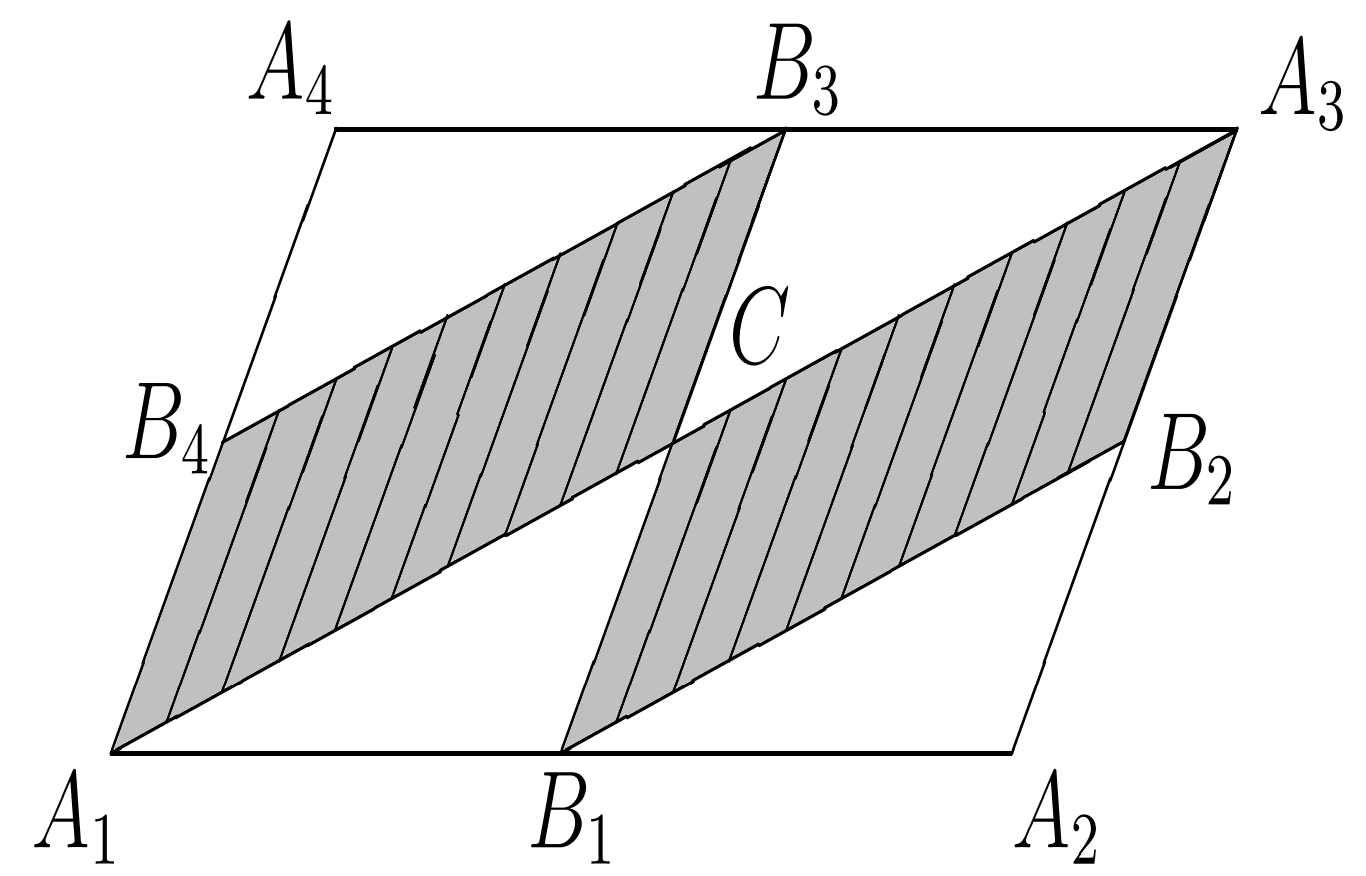
\includegraphics[width=9cm, height=5cm]{passo1grigio.png}
	\centering
	\caption{Figura 1}
	\end{figure}


Ora ripetiamo il procedimento per ciascuno dei nuovi parallelogrammi. Iterando per un numero finito di passi, si ottengono un numero finito di sotto-parallelogrammi di $P$. Nella figura 2 sono mostrati i primi tre passi e sono evidenziati gli otto parallelogrammi ottenuti.\\

\begin{figure} [h!]
	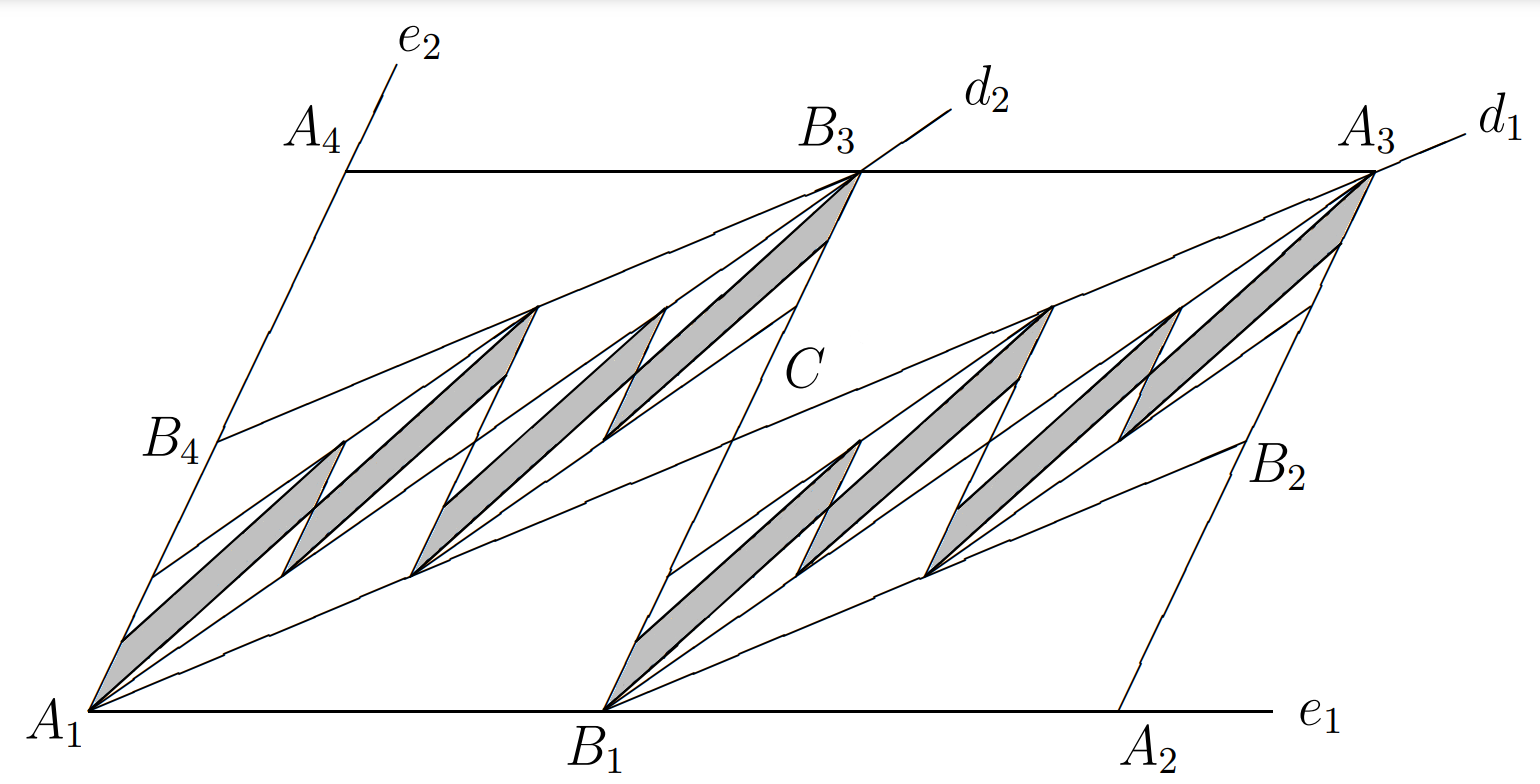
\includegraphics[width=9cm, height=5cm]{passi123grigio.png}
	\centering
	\caption{Figura 2}
\end{figure}

Siano $e_{1}, e_{2}$ le direzioni dei lati di $P$ e siano $d_{1}, d_{2}, \ldots$ le direzioni delle diagonali $A_{1} A_{3}, A_{1} B_{3},...$. Sia ha che $d_{n} \rightarrow e_{2}$.\\
Come illustrato nella figura 3, definiamo dei sottoinsiemi di direzioni come segue. Sia $D_1$ l'insieme delle direzioni delle rette per $A_{4}$ che intersecano $A_{1} A_{3}$; $D_2$ l'insieme di direzioni tra $e_{1}$ e $d_{1}$; $D_3$ l'insieme delle direzioni tra $d_{1}$ e $d_{2}$, ...\\
Notiamo che data una direzione diversa da $e_2$, esiste un $n$ abbastanza grande per cui tale direzione appartiene a $D_n$.

\begin{figure} [h!]
		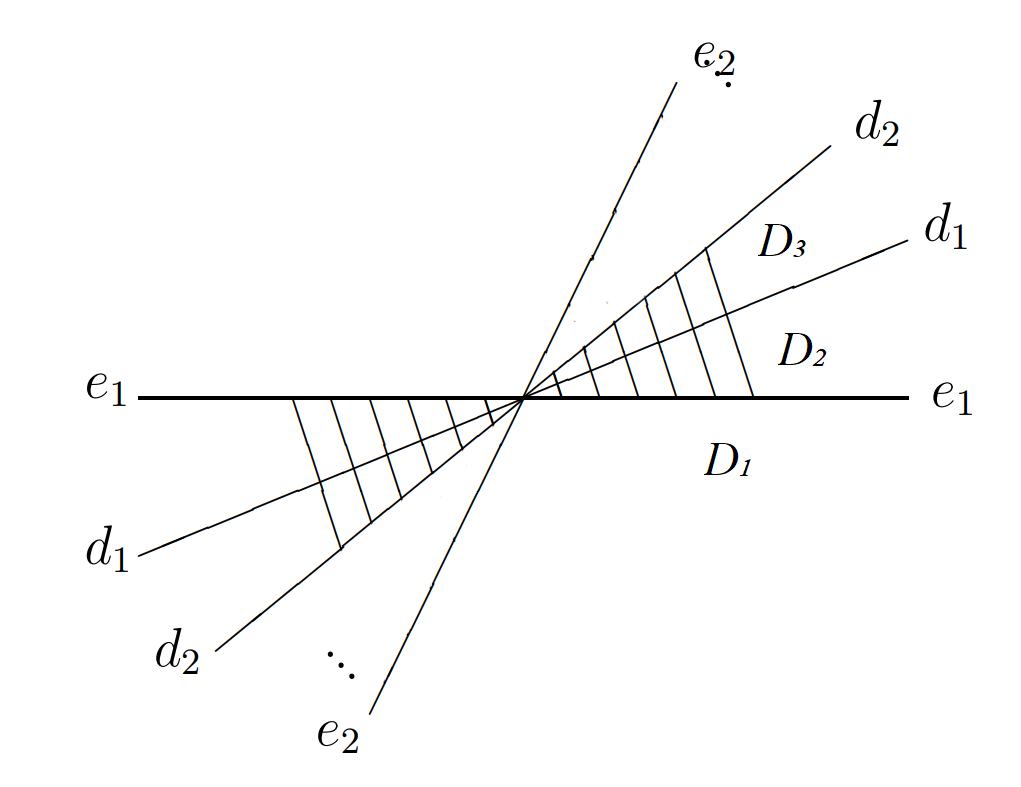
\includegraphics[width=0.6\columnwidth]{direzioni.png}
		\centering
		\caption{Figura 3}
\end{figure}

\textcolor{red}{evidenziare D1}
Ogni retta in direzione appartenente a $D_1$ che interseca $P$ interseca anche la diagonale $A_{1} A_{3}$, quindi uno dei parallelogrammi $A_{1} C B_{3} B_{4}$ e $B_{1} B_{2} A_{3} C$.\\
Inoltre, si vede facilmente che la misura delle proiezioni di ciascuno di questi parallelogrammi sulla retta $A_{1} A_{4}$ è al più $\left|A_{1} A_{4}\right|$ in ogni direzione in $D_2$. Quindi la misura della proiezione dell'unione dei parallelogrammi è al più $2 \cdot\left|A_{1} A_{4}\right|$.\\
Nello stesso modo, ogni retta in direzione in $D_1$ o $D_2$ che interseca $A_{1} C B_{3} B_{4}$ o $B_{1} B_{2} A_{3} C$ interseca uno dei 4 parallelogrammi del secondo passo. Inoltre la misura della proiezione dell'unione dei 4 parallelogrammi sulla retta $A_{1} A_{4}$ nelle direzioni in $D_2 \cup D_3$ è al più $4 \cdot\left|A_{1} B_{4}\right|=2 \cdot\left|A_{1} A_{4}\right|$.\\

Induttivamente, all'$n$-esimo passo, le rette in direzioni appartenenti a $\bigcup_{i=1}^n D_i$ intersecano l'unione dei parallelogrammi costruiti all'$n$-esimo passo, se intersecano uno dei parallelogrammi del passo $n-1$. In particolare una retta in direzione in $D_1$ che interseca $P$, interseca uno dei parallelogrammi dell'$n$-esimo passo.\\
Inoltre la misura della proiezione dell'unione dei parallelogrammi dell'$n$-esimo passo sulla retta $A_{1} A_{4}$ è al più $2 \cdot\left|A_{1} A_{4}\right|$ in ogni direzione in $\bigcup_{i=2}^{n+1}D_i$.\\

\begin{lemma} \label{altroarticolo}
	Sia $I=\left\{I^{1}, I^{2}, \ldots, I^{m}\right\}$ un insieme finito di intervalli due a due disgiunti di direzioni e sia $J=\left\{J^{1}, J^{2}, \ldots, J^{m}\right\}$ un insieme di sotto intervalli stretti (cioè, $\operatorname{cl}\left(J^{j}\right) \subseteq \operatorname{int} I^{j}$ per ogni $j$). Allora per ogni parallelogramma $T$ e $\varepsilon>0$ esistono dei parallelogrammi disgiunti $T_{1}, T_{2}, \ldots \subseteq T$ tali che, detto $U=\bigcup_iT_i$:
	
	\begin{itemize}
		\item per ogni direzione $d \in \bigcup J$ la proiezione di $U$ in direzione $d$ abbia misura minore di $\varepsilon$;
		\item per ogni retta $l$ in direzione $d \notin \bigcup I$, se $l$ interseca $T$ allora $l$ interseca anche $U$.	
	\end{itemize}
\end{lemma}	

\begin{proof}
	Assumiamo $m=1$, con intervalli $J \subseteq I$. Scegliamo un intervallo di direzioni $(a, b)$ tale che $\operatorname{cl}(J) \subsetneq(a, b) \subseteq[a, b] \subsetneq \operatorname{int}(I)$.\\
	Allora possiamo scegliere dei vertici di $T$ e dei parallelogrammi due a due disgiunti in $T$ e tali che:\\
	\textcolor{orange}{forse ho capito perché}
		\begin{itemize}
		\item le direzioni dei lati di tutti i parallelogrammi siano $a$ e $b$;
		\item ogni retta in direzione in $I^c$ che interseca $T$ interseca anche uno dei sotto-parallelogrammi;
		\item la somma dei lati in direzione $a$ sia minore di $\frac{1}{2} \varepsilon$, dove $\varepsilon$ è un numero positivo fissato.
	\end{itemize}	
	Detti questi $\{P_n\}_{n \in \N}$, applichiamo la procedura esposta precedentemente ("venetian blind") ad ogni $P_i$, in modo che il lato $A_1A_4$ sia in direzione $a$, con riferimento alla notazione precedente.\\
	Il numero di passi necessario è indipendente dal $P_i$ scelto ed è dato dalla seguente osservazione: poiché $\operatorname{cl}(J) \subsetneq(a, b)$, esiste $\rho >0$ tale che $J \subseteq (a+\rho,b)$. Quindi esiste un certo $n$ per cui $J \subseteq \bigcup_{i=2}^{n+1}D_i$.\\
	Con questa procedura, per ogni $P_i$, si ottiene una collezione di sotto-parallelogrammi, diciamo $U_i$. Sia allora $U = \bigcup_i U_i$.\\
	La misura della proiezione (non ortogonale) di $U$ sulla retta di direzione $a$ è minore di $2 \cdot \frac{1}{2} \varepsilon=\varepsilon$ in ogni direzione in $J$. Quindi, la misura della proiezione ortogonale in ogni direzione in $J$ è minore di $\varepsilon$.\\
	Infine, considerando il parallelogramma $P_i$ e la sua collezione $U_i$, siccome $D_1 =(a,b)^c$ e $(a,b) \subseteq I$, allora $I^c \subseteq D_1$. Quindi ogni retta in direzione in $I^c$ che interseca $P_i$, interseca anche $U_i$. Quindi ogni retta in direzione in $I^c$ che interseca $T$, interseca anche $U$. \\
\end{proof}
 \textcolor{red}{scambiare I, J, uniformare la notazione tra le varie sezioni}

\newpage

\section{Bibliografia}

[1] \ \ Marianna Cs\"{o}rnyei, "How to make Davies' Theorem visible", 2001\\

[2] \ \ Marianna Cs\"{o}rnyei, "On the visibility of invisible sets", 2000\\

[3] \ \ V. I. Bogachev, "Measure Theory"

\end{document}